\documentclass[twoside,10pt]{article}
\usepackage{/Users/bradenhoagland/latex/styles/toggles}
%\toggletrue{sectionbreaks}
%\toggletrue{sectionheaders}
\newcommand{\docTitle}{HW 4}
\usepackage{/Users/bradenhoagland/latex/styles/common}
\importStyles{modern}{rainbow}{boxy}

%\renewcommand{\theenumi}{\alph{enumi}}

\begin{document}
%\tableofcontents

% ------------------------------
% 1.109
% ------------------------------
\begin{exer}[1.109]
Ptolemy's Theorem.
\end{exer}

\begin{figure}[H]
	\centering
	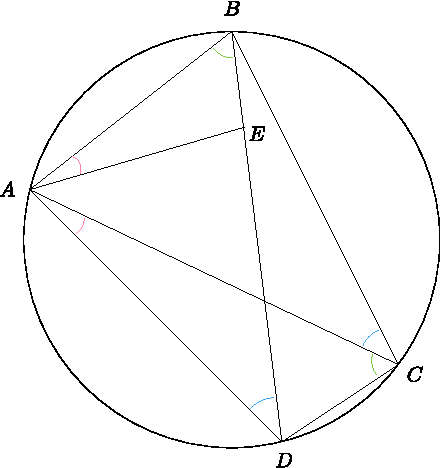
\includegraphics[scale=1]{fig/109.pdf}
	%\caption{}
\end{figure}

By the Star Trek lemma, since $\angle ABD, \angle ACD$ subtend the same arc, they're equal. Then since they have two equal angles, $\Delta ABE \sim \Delta ACD$. Thus
\[
\frac{|AB|}{|AC|} = \frac{|BE|}{|CD|} \implies |AB| |CD| = |AC| |BE|.
\] Similarly, $\Delta ABC \sim \Delta AED$, so
\[
\frac{|AB|}{|AE|} = \frac{|BC|}{|ED|} \implies |BC| |AD| = |AC| |ED|.
\] Adding these two equalities gives
\begin{align*}
	|AB| |CD| + |BC| |AD| &= |AC| (|BE| + |ED|) \\
			      &= |AC| |DB|.
\end{align*}

\newpage

% ------------------------------
% 1.111
% ------------------------------
\begin{exer}[1.111]
Use Ptolemy's Theorem to show the angle sum formula for sines.
\end{exer}

\begin{figure}[H]
	\centering
	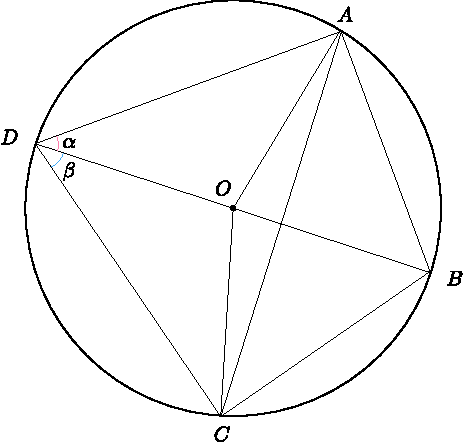
\includegraphics[scale=1]{fig/111.pdf}
	%\caption{}
\end{figure}

In the figure, suppose $BD$ is the diameter, and scale everything so that $|BD|=2$. This means the radius of the circle is one, so the extended law of sines gives
\begin{align*}
	|AC| &= 2 \sin(\alpha+\beta),\\
	|BC| &= 2 \sin \alpha \\
	|AB| &= 2 \sin \beta.
\end{align*}
Now $\angle BAD, \angle DCB$ both subtend half of the circle since $BD$ is the diameter, so both angles are right angles. This means $\Delta ABD$ and $\Delta DBC$ are right triangles with hypotnuse length $|BD|=2$, so
\begin{align*}
	|CD| &= 2 \cos \alpha, \\
	|AD| &= 2 \cos \beta.
\end{align*}
Then by Ptolemy's Theorem,
\begin{align*}
	|AC| |BD| &= |AB| |CD| + |BC| |AD| \\
	\sin(\alpha+\beta) &= \sin \beta \cos \alpha + \sin \alpha \cos \beta.
\end{align*}

\newpage

% ------------------------------
% 1.112
% ------------------------------
\begin{exer}[1.112]
	Cosine formula using sine formula.
\end{exer}

Let $\alpha' = \frac{\pi}{2} -\alpha$ and $\beta'=-\beta$, then by Exercise 1.111,
\begin{align*}
	\sin(\alpha'+\beta') &= \sin \alpha' \cos \beta' + \sin \beta' \cos \alpha' \\
	\sin\left( \frac{\pi}{2} -(\alpha+\beta) \right) &= \sin\left( \frac{\pi}{2} -\alpha \right)\cos(-\beta) + \sin(-\beta) \cos\left( \frac{\pi}{2} -\alpha \right) \\
	\cos(\alpha+\beta) &= \cos \alpha \cos \beta - \sin \beta \sin \alpha.
\end{align*}

\newpage

% ------------------------------
% 1.114
% ------------------------------
\begin{exer}[1.114]
	Angle sum formula for sines and cosines.
\end{exer}

\begin{figure}[H]
	\centering
	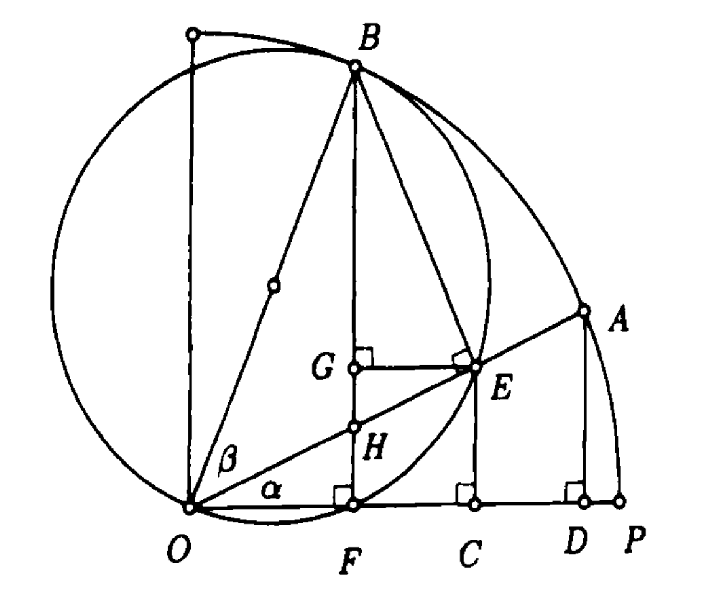
\includegraphics[scale=0.8]{fig/114.pdf}
	%\caption{}
\end{figure}

Scale everything so that $|OB|=1$. Since they share 2 angles, $\Delta OHF \sim \Delta BHE$. In particular, $\angle EBF = \alpha$. Thus $|FC|=|GE|=|BE| \sin (\angle EBF) = \sin \beta \sin \alpha$ and $|OC|=|OE| \cos \alpha = \cos \beta \cos \alpha$. This implies
\[
	\cos(\alpha+\beta) = |OF| = |OC|-|FC| = \cos \beta \cos \alpha - \sin \beta \sin \alpha.
\] 

Similarly, $|BG|=|BE|\cos \alpha = \sin \beta \cos \alpha$ and $|GF|=|EC|=|OE|\sin \alpha = \cos \beta \sin \alpha$. This implies
\[
	\sin(\alpha+\beta) = |BF| = |BG|+|GF| = \sin \beta \cos \alpha + \cos \beta \sin \alpha.
\] 

\newpage

% ------------------------------
% 1.118
% ------------------------------
\begin{exer}[1.118]
IMO hexagon inequality problem.
\end{exer}

\begin{figure}[H]
	\centering
	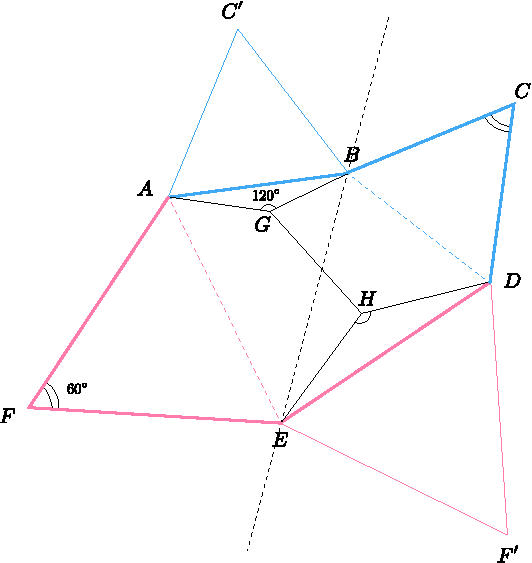
\includegraphics[scale=1]{fig/118.pdf}
	%\caption{}
\end{figure}

Note that $\Delta BCD$ is isosceles with a $60 \degree$ angle, so it's equilateral. Similarly, $\Delta AEF$ is also equilateral (in the diagram all blue lines are the same length and all pink lines are the same length). Then by SSS, $\Delta BDE \cong \Delta BAE$. This means when reflecting over the line $BE$, each of these two triangles will become the other.

First reflect $\Delta BCD$ over $BE$, making the triangle $\Delta C'BA$ (by the previous comment, $BD$ maps perfectly onto $AB$). Since we're given $\angle BGA = 120\degree$ and since we know that the interior angles of an equilateral triangle are all $60\degree$, we have $\angle BGA + \angle AC'B = 180\degree$. Then by Theorem 1.14.1, $C'BGA$ is a cyclic quadrilateral. Now we can use Ptolemy's Theorem to get $|C'G| |AB| = |C'B| |AG| + |GB| |AC'|$. But $|AB|=|C'B|=|AC'|$ since $\Delta C' BA$ is an equialateral triangle, so this simplifies to $|C'G| = |AG| + |GB|$.

Similarly, we can reflect $\Delta FAE$ over $BE$ and follow the same steps to derive $|HF'| = |DH| + |HE|$. Adding these two identities together and adding an extra $|GH|$ on both sides yields
\begin{align*}
	|AG|+|GB|+|DH|+|HE|+|GH| &= |HF'|+|C'G|+|GH| \\
				 &\geq |C'F'| \\
				 &= |CF|,
\end{align*}
where the final equality follows from reflections being isometries.

\newpage

% ------------------------------
% 1.125
% ------------------------------
\begin{exer}[1.125]
Tangents of the incircle are concurrent.
\end{exer}

\begin{figure}[H]
	\centering
	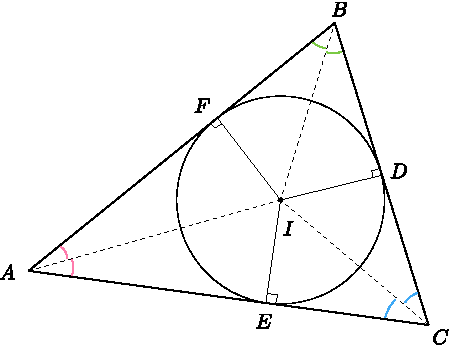
\includegraphics[scale=1]{fig/125.pdf}
	%\caption{}
\end{figure}

By Ceva's Theorem, $AD,BE,CF$ are concurrent $\iff \frac{|AF|}{|FB|} \frac{|BD|}{|DC|} \frac{|CE|}{|EA|} =1$. Now the incenter $I$ is the intersection point of the interior angle bisectors, so all adjacent angles are equal (see the diagram).

	Consider the triangles $\Delta IDC,\Delta IEC$. Due to the equal adjacent angles, $\Delta IDC \sim \Delta IEC$. But since both triangles share a side, they're actually congruent. In particular, $|DC|=|CE|$.

	Similarly, we find $|FB|=|BD|$ and $|AF|=|EA|$. Thus $\frac{|AF|}{|FB|} \frac{|BD|}{|DC|} \frac{|CE|}{|EA|} =1$, so $AD,BE,CF$ are concurrent.

\newpage

% ------------------------------
% 1.129
% ------------------------------
\begin{exer}[1.129]
Intersecting perpendiculars.
\end{exer}

\begin{figure}[H]
	\centering
	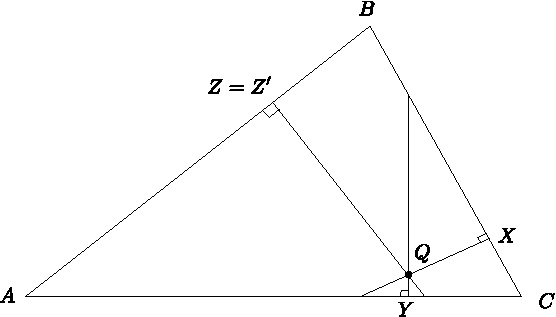
\includegraphics[scale=1]{fig/129.pdf}
	%\caption{}
\end{figure}

\textbf{Concurrency implies the equation:} Suppose the perpendiculars from $X,Y,$ and $Z$ intersect at $Q$. By the Pythagorean Theorem,
\begin{itemize}
	\item $|AQ|^2 = |AZ|^2+|ZQ|^2 = |AY|^2+|YQ|^2$,
	\item $|BQ|^2 = |BX|^2+|XQ|^2 = |BZ|^2+|ZQ|^2$,
	\item $|CQ|^2 = |CY|^2+|YQ|^2 = |CX|^2+|XQ|^2$.
\end{itemize}
Using these identities, $|AZ|^2-|ZB|^2+\left| BX \right|^2-|XC|^2+|CY|^2-|YA|^2=0$.
\vspace{5mm}

\textbf{The equation implies concurrency:} Let
\[
	\mathcal{F}(X,Y,Z) = |AZ|^2-|ZB|^2+\left| BX \right|^2-|XC|^2+|CY|^2-|YA|^2,
\] suppose the perpendiculars from $X$ and $Y$ intersect at a point $ Q$, and suppose $\mathcal{F}(X,Y,Z)=0$. Now drop a perpendicular from $Q$ onto $AB$, and say it lands at a point $Z'$. Then by the other direction of the proof, $X,Y,Z'$ all satisfy the equation.

Without loss of generality, suppose $Z$ sits between $ A$ and $Z'$, then
\begin{align*}
	\mathcal{F}(X,Y,Z) &= \mathcal{F}(X,Y,Z') \\
	|AZ|^2 - |ZB|^2 &= |AZ'|^2 - |Z'B|^2 \\
	|AZ|^2 - (|ZZ'|+|ZB|)^2 &= (|AZ|+|ZZ'|)^2 - |Z'B|^2 \\
	|AZ|^2 - |ZZ'|^2 - 2|ZZ'| |Z'B| - |Z'B|^2 &= |AZ|^2 + 2|AZ| |ZZ'| + |ZZ'|^2 - |Z'B|^2 \\
	|ZZ'|( |AZ|+|ZZ'|+|Z'B|) &= 0 \\
	|ZZ'| |AB| &= 0 \\
	|ZZ'| &= 0,
\end{align*}
where the last equality follows from $|AB|$ being nonzero. Thus $Z=Z'$, so the three perpendiculars intersect.


\newpage

\end{document}
